\documentclass[bachelor, och, labwork]{shiza}

\usepackage{subfigure}
\usepackage{tikz,pgfplots}
\pgfplotsset{compat=1.5}
\usepackage{float}
\usepackage{pdfpages}

\usepackage{titlesec}
\setcounter{secnumdepth}{4}
\titleformat{\paragraph}
{\normalfont\normalsize}{\theparagraph}{1em}{}
\titlespacing*{\paragraph}
{35.5pt}{3.25ex plus 1ex minus .2ex}{1.5ex plus .2ex}

\titleformat{\paragraph}[block]
{\hspace{1.25cm}\normalfont}
{\theparagraph}{1ex}{}
\titlespacing{\paragraph}
{0cm}{2ex plus 1ex minus .2ex}{.4ex plus.2ex}

% --------------------------------------------------------------------------%


\usepackage[T2A]{fontenc}
\usepackage[utf8]{inputenc}
\usepackage{graphicx}
\graphicspath{ {./images/} }
\usepackage{tempora}

\usepackage[sort,compress]{cite}
\usepackage{amsmath}
\usepackage{amssymb}
\usepackage{amsthm}
\usepackage{fancyvrb}
\usepackage{listings}
\usepackage{listingsutf8}
\usepackage{longtable}
\usepackage{array}
\usepackage[english,russian]{babel}

\usepackage[hidelinks]{hyperref}
\usepackage{url}

\usepackage{underscore}
\usepackage{setspace}
\usepackage{indentfirst} 
\usepackage{mathtools}
\usepackage{amsfonts}
\usepackage{enumitem}
\usepackage{tikz}
\usepackage{minted}

\newcommand{\eqdef}{\stackrel {\rm def}{=}}
\newcommand{\specialcell}[2][c]{%
\begin{tabular}[#1]{@{}c@{}}#2\end{tabular}}

\renewcommand\theFancyVerbLine{\small\arabic{FancyVerbLine}}


\begin{document}
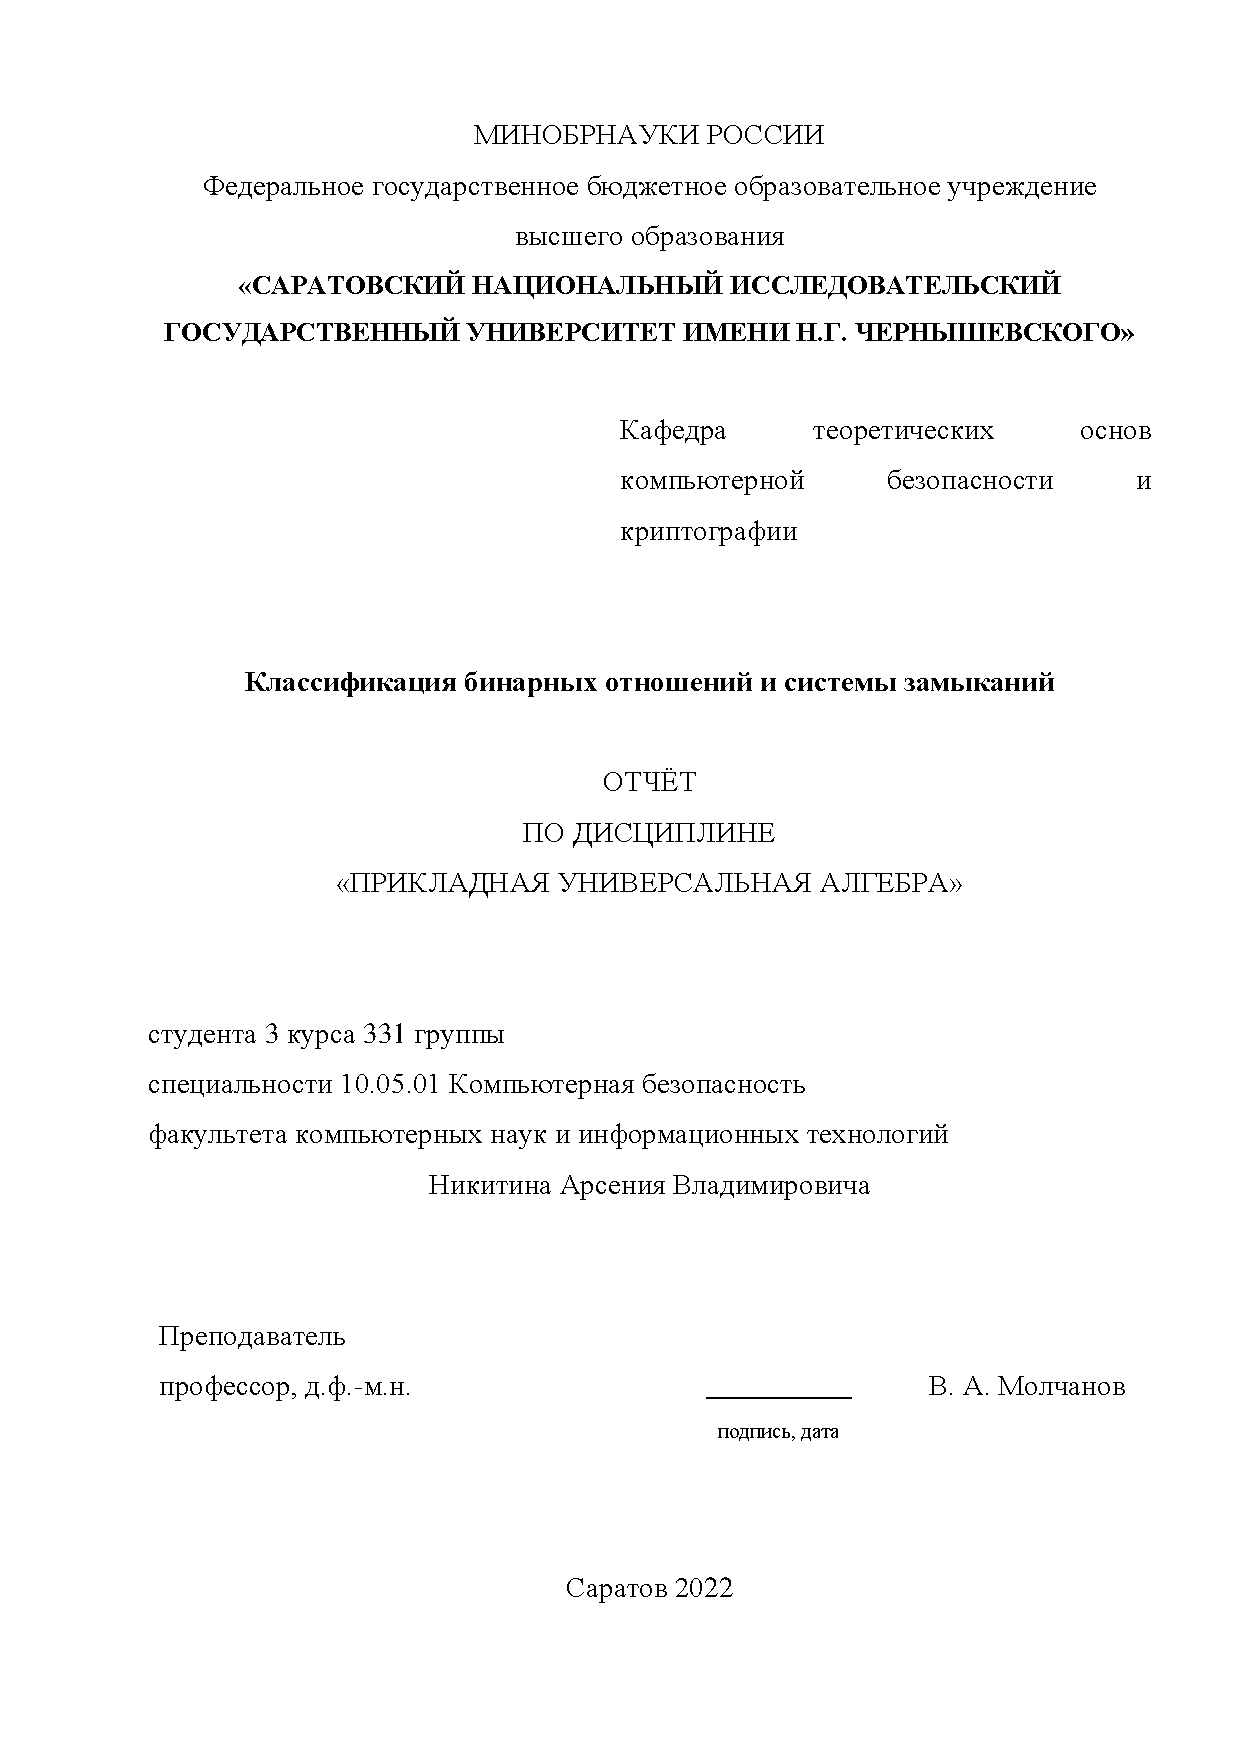
\includepdf{titul.pdf}

%-------------------------------------------------------------------------------

\tableofcontents

\intro

Существует определенная классификация бинарных отношений в зависимости от их 
свойств. Задачей данной работы является рассмотрение основных свойств бинарных 
отношений, а также их классификация. В зависимости от класса бинарного 
отношения, на нем можно определить замыкание: относительно рефлексивности,
симметричности и транзитивности. Для этого требуется понимать, каким образом 
происходит классификация отношений в зависимости от множеств, которыми они могут
задаваться.

\section{\textbf{Цель работы и порядок ее выполнения}}

\textbf{Цель работы} "--- изучение основных свойств бинарных отношений и 
операций замыкания бинарных отношений.

Порядок выполнения работы:

\begin{enumerate}

    \item Разобрать основные определения видов бинарных отношений и разработать
    алгоритм классификации бинарных отношений.

    \item Изучить свойства бинарных отношений и рассмотреть основные системы
    замыкания на множестве бинарных отношений.

    \item Разработать алгоритмы построения основных замыканий бинарных отношений.

\end{enumerate}

\section{Теоретические сведения}

\subsection{Основные определения видов бинарных отношений и их алгоритмы}

\subsubsection{Определение бинарного отношения}

Подмножества декартова произведения $A \times B$ множеств $A$ и $B$ называются
\textbf{бинарными отношениями} между элементами множеств $A$ и $B$ и 
обозначаются строчными греческими буквами $\rho$, $\rho_1$ и т.п.

Для бинарного отношения $\rho\subset A \times B$ область определения $D_\rho$ и 
множество значений $E_\rho$ определяется как подмножества соответствущих множеств 
$A ~\text{и}~ B$ по следующим формулам:

\begin{center}
    $D_\rho ~ = ~ \{a : (a, b) \in\rho ~ \text{для некоторого} ~ b \in B\}$,
    $E_\rho ~ = ~ \{b : (a, b) \in\rho ~ \text{для некоторого} ~ a \in A\}$.
\end{center}

\subsubsection{Основные свойства бинарных и алгоритмы их определения}

Бинарное отношение $\rho \subset A \times A$ называется:

\begin{enumerate}
    
    \item \textit{рефлексивным}, если $(a,a)\in\rho~\forall a \in A$.
    
    \item \textit{антирефлексивным}, если $(a,a)\not\in\rho~\forall a \in A$.
    
    \item \textit{симметричным}, если $(a,b)\in\rho\Rightarrow (b,a)\in\rho~\forall a,b\in A$.
    
    \item \textit{антисимметричным}, если $(a,b) \in\rho~\text{и}~(b,a) \in\rho ~ \Rightarrow a = b ~\forall a,b \in A$.
    
    \item \textit{транзитивным}, если $(a,b)\in\rho ~\text{и}~ (b,c)\in\rho\Rightarrow (a,c) \in\rho ~\forall a,b,c \in A$.

\end{enumerate}

Далее представлена программная реализация определения свойств бинарных 
отношений.

Пусть $\rho$ - бинарное отношение на множестве $A=\{a_1,...,a_N\}$ мощности $N$.
Тогда \textit{матрицей} бинарного отношения $\rho$ будет матрица $M(\rho)$ 
размерности $N \times N$, определяемая следующим образом: 


    \begin{equation*}
        \forall i,j = \overline{1,N} \quad M(\rho)_{ij} = 
            \begin{cases}
                1, &\text{если $(a_i,a_j) \in \rho$}\\
                0, &\text{если  $(a_i,a_j) \not\in \rho$}
            \end{cases}
    \end{equation*}


Выполним проверку свойств \textbf{рефлексивности} и \textbf{антирефлексивности}:

Алгоритм 1. Проверка бинарного отношения на \textit{рефлексивность}.

\textit{Вход.} Матрица $M(\rho)$ бинарного отношения $\rho$ размерности
$N \times N$.

\textit{Выход.} <<Отношение является рефлексивным>> или "Отношение не является 
рефлексивным".

\begin{enumerate}
        
    \item Цикл по $i ~\text{от}~ 1 ~\text{до}~ N$.

    \item Если $M_{ii} = 0$, то ответ <<Отношение не является рефлексивным>>. 

    \item Если цикл завершен то ответ <<Отношение является рефлексивным>>.
    
\end{enumerate}
Трудоемкость алгоритма $O(n)$.

Алгоритм 2. Проверка бинарного отношения на \textit{антирефлексивность}.

\textit{Вход.} Матрица $M(\rho)$ бинарного отношения $\rho$ размерности
$N \times N$.

\textit{Выход.} <<Отношение является антирефлексивным>> или <<Отношение не является 
антирефлексивным>>.

\begin{enumerate}
        
    \item Цикл по $i ~\text{от}~ 1 ~\text{до}~ N$.

    \item Если $M_{ii} = 1$, то ответ "Отношение не является антирефлексивным. 

    \item Если цикл завершен то ответ "Отношение является антирефлексивным.
    
\end{enumerate}
Трудоемкость алгоритма $O(n)$.

Выполним проверку свойств \textbf{симметричности и антисимметричности}:

Свойство симметричности выполняется для отношения, заданного матрицей, если
элементы, симметричные относительно главной диагонали равны.

Алгоритм 3. Проверка бинарного отношения на \textit{симметричность}.

\textit{Вход.} Матрица $M(\rho)$ бинарного отношения $\rho$ размерности
$N \times N$.

\textit{Выход.} <<Отношение является симметричным>> или <<Отношение не является
симметричным>>.

\begin{enumerate}
    \item Цикл по $i ~\text{от}~ 1 ~\text{до}~ N$, 
    цикл по $j ~\text{от}~ 1 ~\text{до}~ N$.

    \item Если $M_{ij} \not= M_{ji}$, то ответ <<Отношение не является симметричным>>.
    
    \item Если циклы завершены, то ответ <<Отношение является симметричным>>.

\end{enumerate}
Трудоемкость алгоритма $O(N^2)$.

Алгоритм 4. Проверка бинарного отношения на \textit{антисимметричность}.

\textit{Вход.} Матрица $M(\rho)$ бинарного отношения $\rho$ размерности
$N \times N$.

\textit{Выход.} <<Отношение является антисимметричным>> или <<Отношение не является
антисимметричным>>.

\begin{enumerate}
    \item Цикл по $i ~\text{от}~ 1 ~\text{до}~ N$, 
    цикл по $j ~\text{от}~ 1 ~\text{до}~ N$.

    \item Если $M_{ij} = M_{ji} = 1 ~\text{и}~ j \ne i$, то ответ <<Отношение не является антисимметричным>>.
    
    \item Если циклы завершены, то ответ <<Отношение является антисимметричным>>.

\end{enumerate}
Трудоемкость алгоритма $O(N^2)$.

Выполним проверку свойства \textbf{транзитивности}:

Свойство транзитивности выполняется для отношения, заданного матрицей, если для 
любого фиксированного элемента $M_{k,i}=1$ из матрицы отношения, и для любого
элемента из матрицы отношения $M_{i,j}=1$, то выполняется $M_{k,j}=1$.

Алгоритм 5. Проверка бинарного отношения на \textit{транзитивность}.

\textit{Вход.} Матрица $M(\rho)$ бинарного отношения $\rho$ размерности
$N \times N$.

\textit{Выход.} <<Отношение является транзитивным>> или <<Отношение не является
транзитивным>>.

\begin{enumerate}
    
    \item Цикл по $k ~\text{от}~ 1 ~\text{до}~ N$, 
    цикл по $i ~\text{от}~ 1 ~\text{до}~ N$, цикл по $j ~\text{от}~ 1 ~\text{до}~ N$.
    
    \item Если $M_{k,i}=M_{i,j}=1 ~\text{и}~ M_{k,j}=0$, то ответ <<Отношение не является
    транзитивным>>.
   
    \item Если циклы завершены, то ответ <<Отношение не является транзитивным>>

\end{enumerate}
Трудоемкость алгоритма $O(N^3)$.

\subsection{Классификация бинарных отношений}

Таким образом, в зависимости от свойств, которыми заданное бинарное отношение
обладает, его можно отнести к определенному классу: \textbf{квазипорядка,
эквивалентности} или \textbf{частичного порядка}. 

\subsubsection{Определения классов бинарных отношений}

Отношение \textit{эквивалентности} -- это такое бинарное отношение между элементами
множества $A$, для которого выполнены свойства рефлексивности, симметричности 
и транзитивности.

Отношение \textit{квазипорядка} -- это такое бинарное отношение, между элементами
множества $A$, для которого выполнены свойства рефлексивности и транзитивности.

Отношение \textit{частичного порядка} -- это такое бинарное отношение, между
элементами множества $A$, для которого выполнены свойства рефлексивности, 
транзитивности и антисимметричности.

\subsubsection{Алгоритм проверки отношения на квазипорядок}

\textit{Вход.} Матрица $M(\rho)$ бинарного отношения $\rho$ размерности
$N \times N$.

\textit{Выход.} <<Отношение является отношением квазипорядка>> или <<Отношение 
не является отношением квазипорядка>>.

\begin{enumerate}

    \item Запустить проверку свойств рефлексивности и транзитивности и выполнить
    логическую операцию \& для их результатов.

    \item Если значение \textit{Истина}, то ответ <<Отношение является отношением
    квазипорядка>>.
    
    \item Если значение \textit{Ложь}, то ответ <<Отношение не является 
    отношением квазипорядка>>.

\end{enumerate}
Трудоемкость алгоритма $O(N+N^3) = O(N^3)$ в силу запуска алгоритмов проверки
свойств рефлексивности и транзитивности.

\subsubsection{Алгоритм проверки отношения на эквивалентность}

\textit{Вход.} Матрица $M(\rho)$ бинарного отношения $\rho$ размерности
$N \times N$.


\textit{Выход.} <<Отношение является отношением эквивалентности>> или 
<<Отношение не является отношением эквивалентности>>.

\begin{enumerate}

    \item Запустить проверку свойств рефлексивности, транзитивности и симметричности
    и выполнить операцию \& для их результатов.

    \item Если получившееся значение истинно, то ответ <<Отношение является
    отношением эквивалентности>>.

    \item Если же значение ложно, то ответ <<Отношение не является отношением
    эквивалентности>>. 

\end{enumerate}
Трудоемкость алгоритма $O(N+N^3+N^2) = O(N^3)$ в силу запуска алгоритмов проверки
свойств рефлексивности, транзитивности и симметричности.

\subsubsection{Алгоритм проверки отношения на частичный порядок}

\textit{Вход.} Матрица $M(\rho)$ бинарного отношения $\rho$ размерности
$N \times N$.

\textit{Выход.} <<Отношение является
отношением частичного порядка>> или <<Отношение не является отношением 
частичного порядка>>.

\begin{enumerate}
    
    \item Запустить проверку свойств рефлексивности, транзитивности и 
    антисимметричности и выполнить операцию \& для их результатов.
    
    \item Если получившееся значение истинно, то ответ <<Отношение является
    отношением частичного порядка>>.
    
    \item Если же получившееся значение ложно, то ответ <<Отношение является
    отношением частичного порядка>>.

\end{enumerate}
Трудоемкость алгоритма $O(N+N^3+N^2) = O(N^3)$ в силу запуска алгоритмов проверки
свойств рефлексивности, транзитивности и антисимметричности.

\subsection{Замыкания бинарных отношений и алгоритмы их построения}

\subsubsection{Определение замыканий отношения}

\textbf{Замыканием отношения} $R$ относительно свойства $P$ называется такое
множество $R^*$, что:

\begin{enumerate}

    \item $R \subset R^*$.

    \item $R^*$ Обладает свойством $P$.

    \item $R^*$ является подмножеством любого другого отношения, содержащего $R$
    и обладающего свойством $P$. 

    То есть $R^*$ является минимальным надмножеством множества $R$, 
    выдерживается $P$.

\end{enumerate}

Итак, исходя из вышесказанного, можно сделать вывод, что существуют 4 вида 
замыканий отношений: \textbf{транзитивное, симметричное, рефлексивное и
эквивалентное}.

На множестве $P(A^2)$ всех бинарных отношений между элементами множества $A$ 
следующие отображения являются операторами замыканий:
\begin{enumerate}
    \item $f_r(\rho) = \rho ~\cup \vartriangle_A$ -- наименьшее рефлексивное
    бинарное отношение, содержащее отношение $\rho \subset A^2$. 
    \item $f_s(\rho) = \rho \cup \rho^{-1}$ -- наименьшее симметричное
    бинарное отношение, содержащее отношение $\rho \subset A^2$.
    \item $f_t(\rho) = \cup^{\infty}_{n=1} \rho^n$ -- наименьшее транзитивное
    бинарное отношение, содержащее отношение $\rho \subset A^2$.
    \item $f_{eq}(\rho) = f_tf_sf_r(\rho)$ -- наименьшее отношение эквивалентности,
    содержащее отношение $\rho \subset A^2$.
    
\end{enumerate}
\subsubsection{Пример построения замыканий бинарного отношения}

Рассмотрим множество $A=$ \{1,2,3,4\}, на котором задано отношение 
$R=$ {(1,2),(3,4),(4,2)} 

\begin{enumerate}

    \item Замыканием $R$ относительно свойства \textbf{рефлексивности}:
        \begin{center}

            $R^*=$ \{(1,2),(3,4),(4,2);(1,1),(2,2),(3,3),(4,4)\} 
        
        \end{center}
  
    \item Замыканием $R$ относительно свойства \textbf{симметричности}: 
        \begin{center}
    
            $R^*=$ \{(1,2),(3,4),(4,2);(2,1),(2,4),(4,3)\} 
    
        \end{center}
  
    \item Замыканием $R$ относительно свойства \textbf{транзитивности}: 
        \begin{center}
        
            $R^*=$ \{(1,2),(3,4),(4,2);(3,2)\} 
        
        \end{center}

\end{enumerate}



\subsubsection{Алгоритм построения рефлексивного замыкания}

% Для этого выполним циклический обход по всем элементам главной диагонали 
% матрицы отношения $M_{ij}$ и будем проверять, находится ли элемент 
% $(M_{ii},M_{ii})$ в исходном отношении.

\textit{Вход.} Матрица $M(\rho)$ бинарного отношения $\rho$ размерности
$N \times N$.

\textit{Выход.} Замыкание относительно свойства рефлексивности.

\begin{enumerate}
    \item Создать пустой список для хранения пар замыкания, а также использовать
    глобальное множество для хранения пар замыкания относительно эквивалентности.
    \item Цикл по $i ~\text{от}~ 1 ~\text{до}~ N$.
    \item Если $M_{ii} = 0$, пару $(i, i)$ добавить в замыкание 
    рефлексивности.
    \item Ответ - замыкание бинарного отношения $\rho$ относительно рефлексивности.
\end{enumerate}
Трудоемкость алгоритма $O(N)$


\subsubsection{Алгоритм построения симмметричного замыкания}

% Для этого выполним циклический обход по всем элементам матрицы 
% отношения $M(\rho)$ и будем проверять, равны ли между собой элементы 
% $M_{ij},M_{ji}$ в исходном отношении.

\textit{Вход.} Матрица $M(\rho)$ бинарного отношения $\rho$ размерности
$N \times N$.

\textit{Выход.} Замыкание бинарного отношения $\rho$ относительно свойства симметричности.

\begin{enumerate}
    \item Создать пустой список для хранения пар замыкания, а также использовать
    глобальное множество для хранения пар замыкания относительно эквивалентности.
    \item Цикл по $i ~\text{от}~ 1 ~\text{до}~ N$, цикл по $j ~\text{от}~ 1 ~\text{до}~ N$.
    \item Если $M_{ij} = 1 ~\text{и}~ M_{ji} = 0$, добавить пару $(j, i)$
    в замыкание симметричности.
    \item Ответ - замыкание бинарного отношения $\rho$ относительно симметричности.
\end{enumerate}
Трудоемкость алгоритма $O(N^2)$


\subsubsection{Алгоритм построения транзитивного замыкания}
% Выполним построение замыкания отношения относительно свойства транзитивности.

% Выполним циклический обход по всем элементам матрицы $M_{ij}$ со всеми
% фиксированными элементами $M_{ki}$:

\textit{Вход.} Матрица $M(\rho)$ бинарного отношения $\rho$ размерности
$N \times N$.

\textit{Выход.} Замыкание бинарного отношения $\rho$ относительно свойства транзитивности.

\begin{enumerate}
    \item Создать копию матрицы исходного бинарного отношения.
    \item Цикл по $e ~\text{от}~ 1 ~\text{до}~ N$, цикл по $k ~\text{от}~ 1 ~\text{до}~ N$, 
    цикл по $i ~\text{от}~ 1 ~\text{до}~ N$, цикл по $j ~\text{от}~ 1 ~\text{до}~ N$.
    \item Если $M_{ki}=M_{i,j}=1 ~\text{и}~ M_{kj}=0$, то добавить пару
    $(k, j)$ в замыкание транзитивности.
    \item Ответ - замыкание бинарного отношения $\rho$ относительно транзитивности.
\end{enumerate}
Трудоемкость алгоритма $O(N^4)$


\subsubsection{Алгоритм построения эквивалентного замыкания}

\textit{Вход.} Матрица $M(\rho)$ бинарного отношения $\rho$ размерности
$N \times N$.

\textit{Выход.} Эквивалентное замыкание бинарного отношения $\rho$.

% Выполним построение замыкания отношения относительно эквивалентности.

\begin{enumerate}
    \item По очереди вызвать алгоритмы построения замыканий относительно рефлексивности,
    симметричности и транзитивности.
    \item Ответ - эквивалентное замыкание бинарного отношения $\rho$.
\end{enumerate}
Трудоемкость алгоритма $O(N+N^4+N^2) = O(N^4)$ в силу вызова алгоритмов построения
замыканий относительно рефлексивности, симметричности и транзитивности

\section{Программная реализация рассмотренных алгоритмов}
    
    \subsection{Результаты тестирования программы}

        \begin{figure}[H]
            \centering
            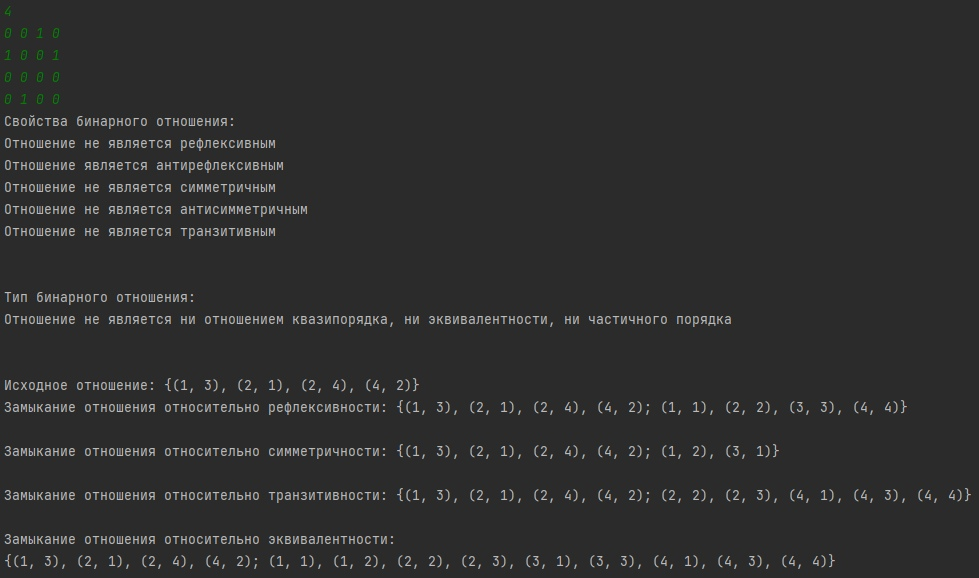
\includegraphics[width=0.8\textwidth]{pic/1.jpg}
            \caption{}
        \end{figure}
    
    \subsection{Код программы, реализующей рассмотренные алгоритмы}
    
        \inputminted[linenos,breaklines=true, fontsize=\small, style=bw]{python}{code/lab1.py}

\conclusion
В ходе лабораторной работы были рассмотрены основные свойства бинарных отношений:
рефлексивность, антирефлексивность, симметричность, антисимметричность и 
транзитивность. По определенным комбинациям свойств отношений, их можно 
классифицировать, как отношения квазипорядка (если отношение обладает 
свойствами транзитивности и рефлексивности), эквивалентности (если отношение 
является отношением квазипорядка, а также имеет свойство симметричности), а 
также отношения частичного порядка (если отношение является отношением 
квазипорядка и имеет свойство антисимметричности). Также были разработаны 
алгоритмы определения свойств отношений и их классификации. В ходе работы стало 
понятно, что самым ресурсоемким стал алгоритм определения транзитивности 
отношения, так как его реализация включает в себя тройной вложенный цикл.

\end{document}